\section{Введение}

Для определения величины отношения заряда электрона к постоянной Больцмана в данной работе используется метод, основанный на исследовании процессов, протекающих в биполярном транзисторе.

\subsection{Решаемые задачи}

\begin{enumerate}
    \item Измерить зависимость тока короткого замыкания коллектора биполярного транзистора от напряжения между эмиттером и базой.
    \item По результатам измерений определить отношение заряда электрона к постоянной Больцмана.
\end{enumerate}

\section{Основная часть}

\subsection{Теоретическая часть}

\subsubsection{Основы p-n перехода и его свойства}

p-n переход формируется на границе соприкосновения двух типов полупроводниковых материалов:
\begin{itemize}
\item Полупроводник n-типа ("донорный"), который создаётся путём легирования 4-валентного полупроводника (кремний, германий) 5-валентными примесями (мышьяк), что приводит к появлению избыточных электронов.
\item Полупроводник p-типа ("акцепторный"), который образуется при введении 3-валентных примесей (бор), создающих "дырки" - вакантные места для электронов.
\end{itemize}

В зоне контакта этих материалов формируется обеднённая область и происходят следующие процессы:
\begin{enumerate}
\item Диффузия носителей: процесс перемещения электронов n-области в p-область и движения дырок из p-области в n-область создаёт диффузионный ток.
\item Образование пространственного заряда: у границы p-области накапливается избыток электронов, а у границы n-области — их дефицит. Эти нескомпенсированные заряды создают внутреннее электрическое поле.
\item Установление равновесия: Возникает дрейфовый ток, противоположный диффузионному, при равновесии токи компенсируют друг друга, и формируется обеднённая область с минимальной концентрацией свободных носителей.
\end{enumerate}

Важной особенностью p-n перехода является его односторонняя проводимость, проявляющаяся при внешнем смещении:
\begin{itemize}
\item Прямое смещение: Внешнее поле противоположно внутреннему и компенсирует его, диффузионный ток резко возрастает, обеднённый слой уменьшается, а переход находится в открытом состоянии.
\item Обратное смещение: Внешнее поле усиливает внутреннее, диффузионный ток крайне мал, обеднённый слой расширяется, переход находится в закрытом состоянии.
\end{itemize}

\subsubsection{Принцип работы биполярного транзистора}

Биполярный транзистор представляет собой трехслойную полупроводниковую структуру (эмиттер, база и коллектор) с двумя близко расположенными p-n переходами и чередующимися типами проводимости. Существует два основных типа: n-p-n транзистор, используемый в данной работе, и p-n-p транзистор. Каждый слой имеет свои особенности: эмиттер имеет наибольшую степень легирования, база -- самая узкая и слаболегированная область, коллектор самый большой по своим размерам.

В данной работе исследуется схема включения с общей базой, где база является общим электродом для входной и выходной цепей, эмиттерный переход смещён в прямом направлении (малое входное сопротивление), а коллекторный — в обратном (большое выходное сопротивление).

Благодаря прямому смещению эмиттерного перехода снижается потенциальный барьер, и электроны из эмиттера инжектируются в базу. Большинство электронов достигают коллекторного перехода за счёт малой толщины базы, высокой концентрации дырок в ней и из-за её слабой легированности. Обратное смещение коллекторного перехода создаёт условия для эффективного сбора электронов коллектором, формируя коллекторный ток.

\subsubsection{Математическая модель}

Ток коллектора $I_k$ в схеме с общей базой описывается уравнением:
\begin{equation}
\label{eq:1}
   I_k = I_0 \left( e^{\frac{eU_{\text{эб}}}{kT}} - 1 \right)
\end{equation}
где $I_0$ — ток насыщения, $e$ — заряд электрона, $k$ — постоянная Больцмана, $T$ — температура (K), $U_{\text{эб}}$ — напряжение между эмиттером и базой.

При комнатной температуре и напряжении $U_{\text{эб}} \approx 0.5{-}1.0\,\text{В}$ экспоненциальный член значительно превосходит единицу, что позволяет упростить уравнение ~\ref{eq:1} до:

\begin{equation}
\label{eq:2}
   I_k = I_0e^{\frac{eU_{\text{эб}}}{kT}}
\end{equation}

Прологарифмировав уравнение ~\ref{eq:2}, получаем линейную зависимость:

\begin{equation}
\label{eq:3}
   \ln I_k = \ln I_0 + \frac{e}{kT}U_{\text{эб}}
\end{equation}

Выражение ~\ref{eq:3} представляет собой уравнение прямой с наклоном $ \tg \alpha = \frac{e}{kT}$. Таким образом, искомое соотношение:

\begin{equation}
\label{eq:4}
   \frac{e}{k} = T \tg \alpha
\end{equation}

Это отношение можно найти, построив зависимость $\ln I_k$ от $U_{\text{эб}}$ и определив $\tg \alpha$ из уравнения ~\ref{eq:3}. Так как нам неизвестно значение $I_0$, требуется система из двух уравнений, однако этот вариант обладает существенными недостатками: высокая чувствительность к погрешностям измерений $U_{\text{эб}}$ и $U_{\text{эб}}$ и риск получения некорректного результата при выходе точек за пределы области применимости модели. Наиболее надежным является метод наименьших квадратов, позволяющий минимизировать влияние случайных погрешностей. Для приближенных расчетов может быть использован метод парных точек.

\subsection{Эксперимент}
На рис.~\ref{fig:photo} представлена фотография электрической установки с биполярным транзистором n-p-n типа. В ней используются: цифровые вольтметры, источник электрического питания УПУ-1У4, транзистор П702А. Схема электрической установки приведена на рис.~\ref{fig:scheme}. На ней "БП"\verb|,| блок питания (УПУ-1У4) — источник постоянного напряжения, V1 и V2 — цифровые вольтметры для измерения $U_{\text{эб}}$ и $U_{\text{кб}}$ соответственно, R1 — ограничительный резистор, R2 — потенциометр, с помощью которого можно изменять напряжение $U_{\text{эб}}$, R3 — резистор в цепи коллектор-база для измерения $I_k$.

Эксперимент заключается в измерении напряжения $U_{\text{кб}}$ в зависимости от подаваемого значения $U_{\text{эб}}$, которое вводится с помощью потенциометра R2 в пределах $0.30{-}0.45$ с шагом 0.01 В. Эксперимент проводится дважды: сначала с точностью вольтметра V1 до 2 знаков после запятой, а потом с точностью до 4 знаков после запятой. Точность для вольтметра V2 постоянная — 4 знака после запятой. Для резистора R3 было выбрано сопротивление, равное 12 Ом. Была измерена температура  в лаборатории: $t = {23 \pm 0.5}{^\circ}C$ или $T = {296,15 \pm 0.5}K$.

\begin{figure}[H]
\centering
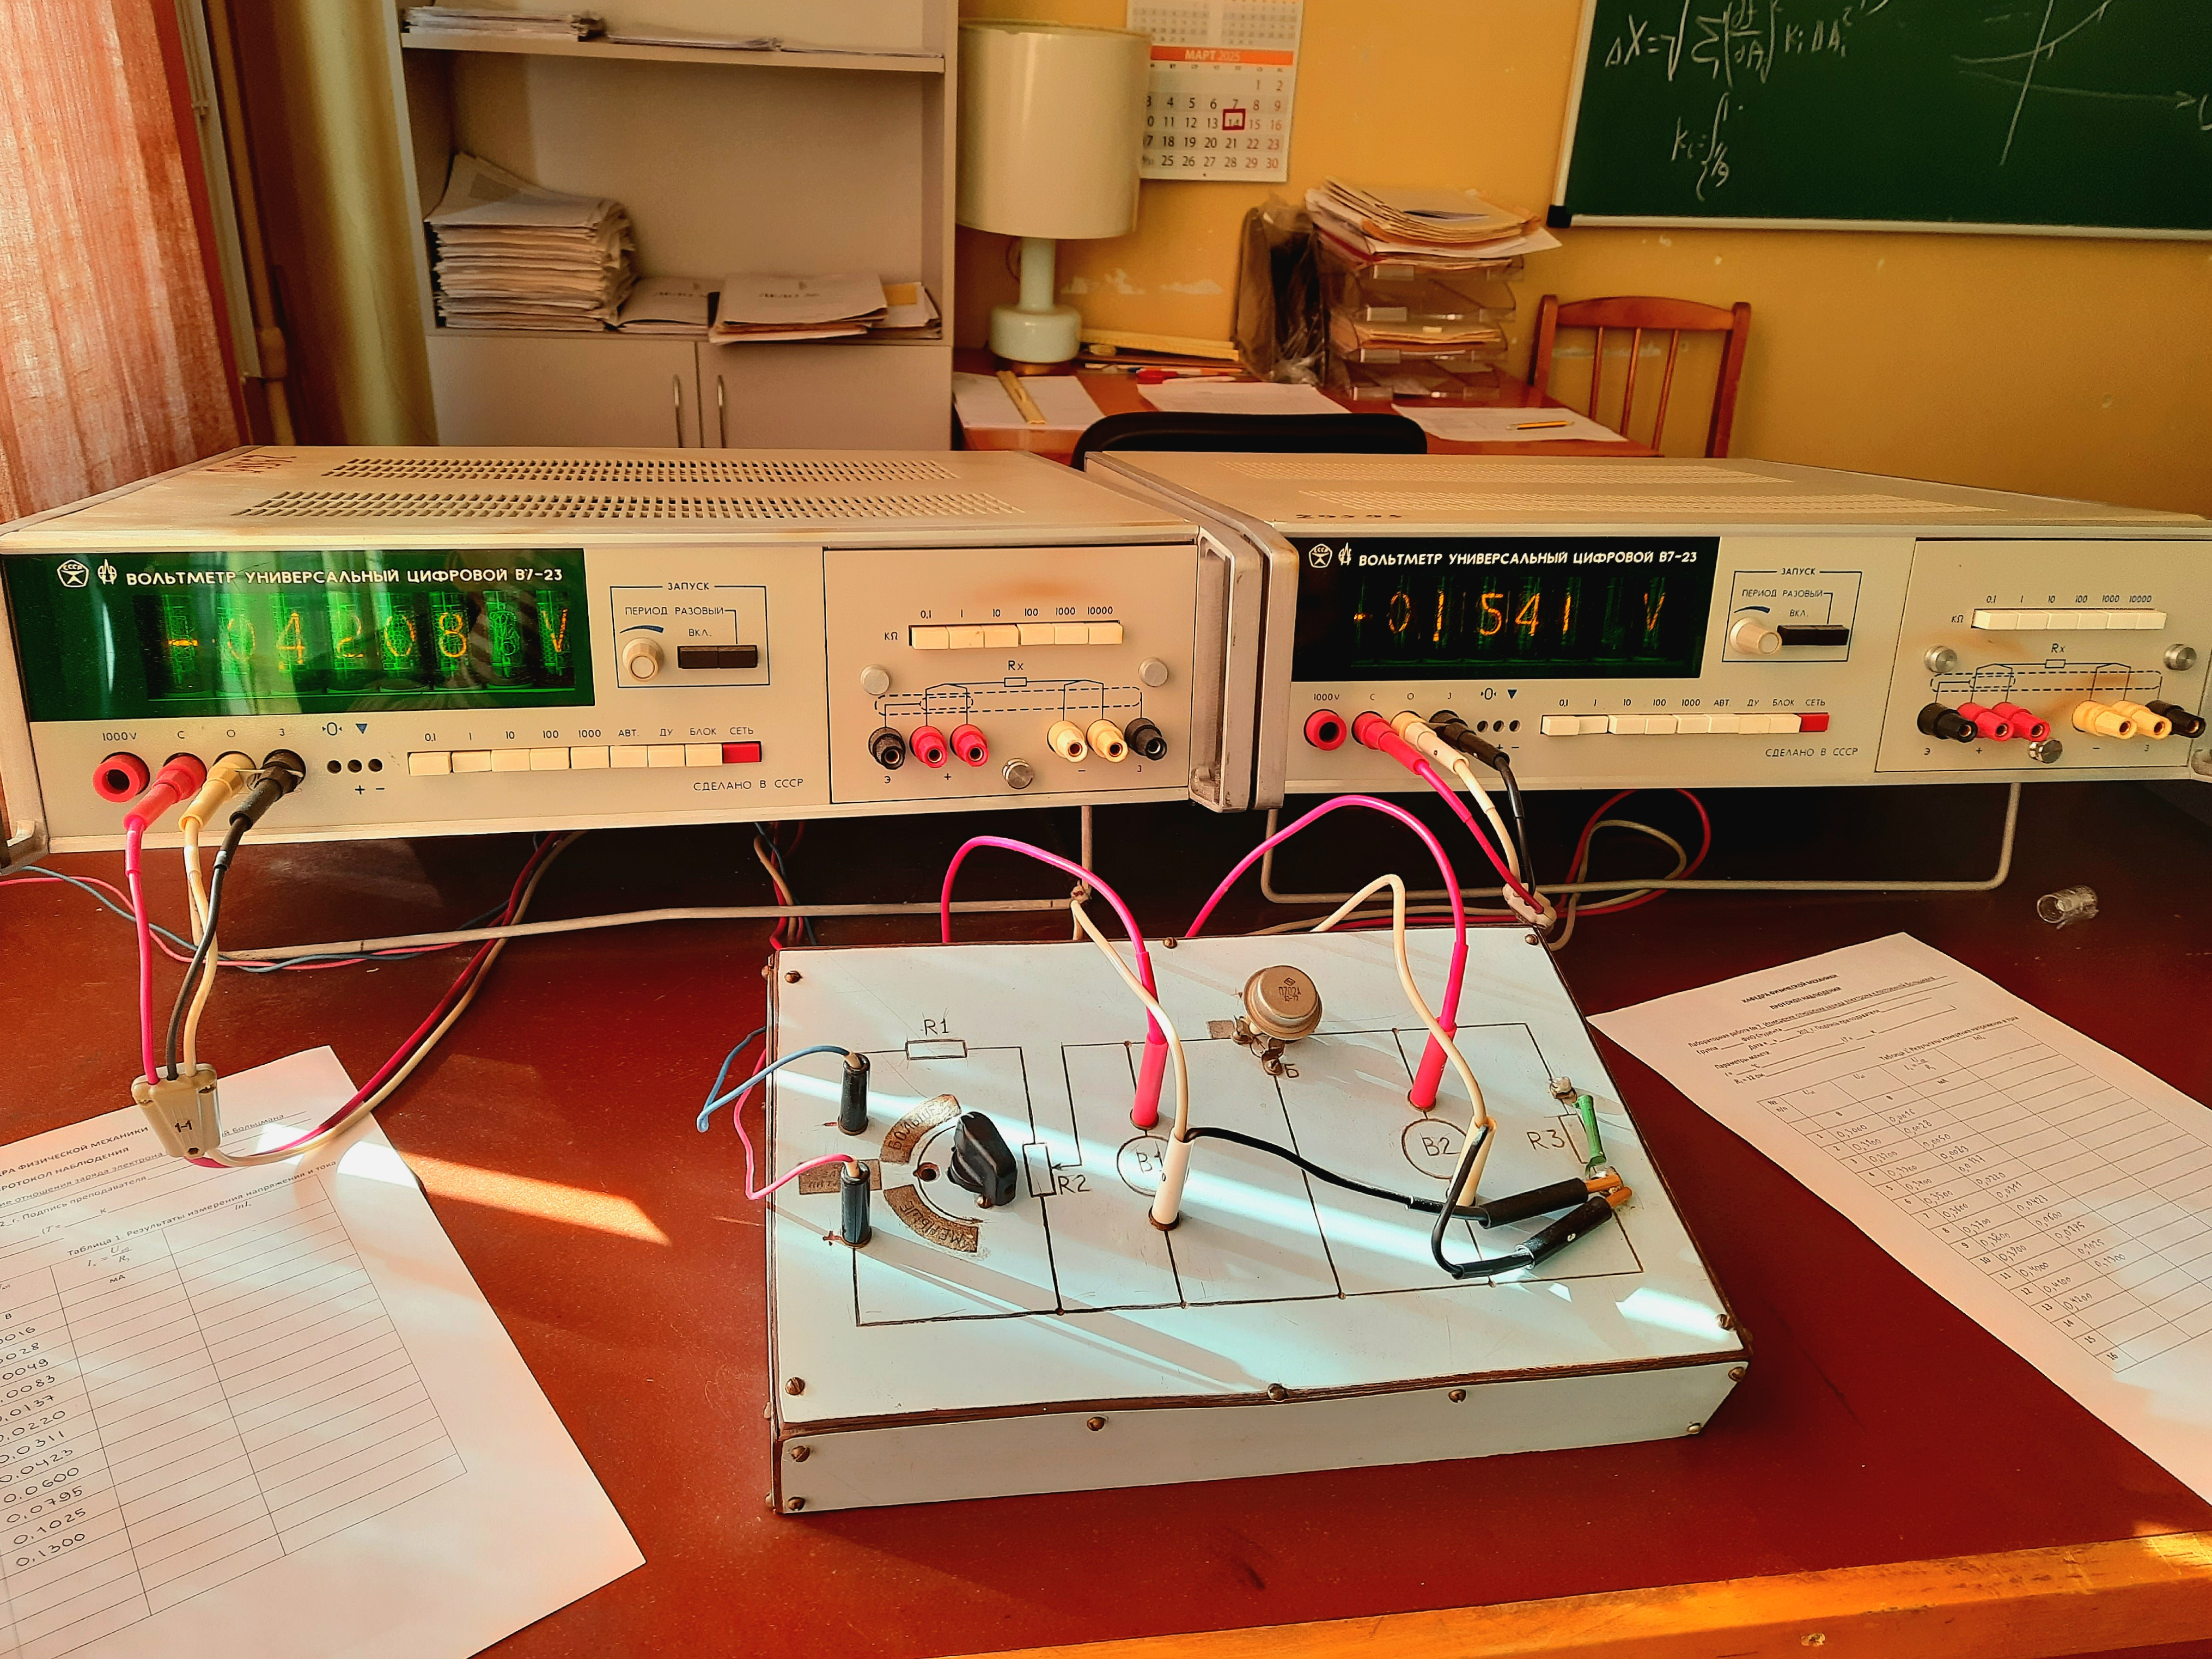
\includegraphics[width=0.8\textwidth]{photo.jpg}
\caption{Фотография электрической установки}
\label{fig:photo}
\end{figure}

\begin{figure}[H]
\centering
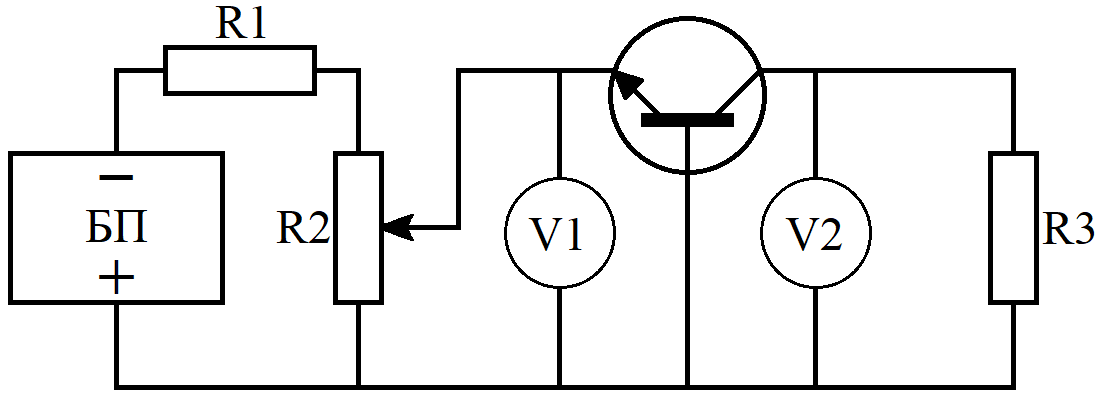
\includegraphics[width=0.9\textwidth]{scheme.png}
\caption{Схема электрической установки}
\label{fig:scheme}
\end{figure}

\subsection{Обработка данных и обсуждение результатов}
 
\subsubsection{Таблицы}

В ходе работы было проведено по 16 измерений напряжения с разными точностями измерения напряжения вольтметра V1. В таблице \hyperref[tab:1]{1} — с точностью до 2 знаков после запятой, а в таблице \hyperref[tabl:1]{1'} — с точностью до 4 знаков после запятой.

\begin{center}
\begin{table}[H]
\centering
\caption*{Таблица 1. Результаты измерения напряжения и тока}
\label{tabl:1}
\begin{tabular}{|c|c|c|c|c|}
\hline
\begin{minipage}{7mm}
    № п.п. 
\end{minipage}&
\begin{minipage}{3.8cm}
    \begin{center}
    $U_{\text{эб}}$
    \end{center}
\end{minipage} &
\begin{minipage}{3.8cm}
    \begin{center}
    $U_{\text{кб}}$
    \end{center}
\end{minipage} &
\begin{minipage}{3.8cm}
    \begin{center}
    $I_{\text{к}}=\frac{U_{\text{кб}}}{R3}$
    \end{center}
\end{minipage}&
\begin{minipage}{3.8cm}
   \begin{center}
   $\ln I_k$
   \end{center}
\end{minipage}\\
\hline
{}&В&В&мА&-\\
\hline
1  & 0.30 & 0.0020 & 0.17 & -1.8   \\
2  & 0.31 & 0.0028 & 0.23 & -1.5   \\
3  & 0.32 & 0.0048 & 0.4  & -0.92  \\
4  & 0.33 & 0.0112 & 0.93 & -0.073 \\
5  & 0.34 & 0.0162 & 1.4  & 0.34   \\
6  & 0.35 & 0.0255 & 2.1  & 0.74   \\
7  & 0.36 & 0.0362 & 3.0  & 1.1    \\
8  & 0.37 & 0.0470 & 3.9  & 1.4    \\
9  & 0.38 & 0.0745 & 6.2  & 1.8    \\
10 & 0.39 & 0.0940 & 7.8  & 2.1    \\
11 & 0.40 & 0.1215 & 10   & 2.3    \\
12 & 0.41 & 0.1490 & 12   & 2.5    \\
13 & 0.42 & 0.1560 & 13   & 2.6    \\
14 & 0.43 & 0.1975 & 16   & 2.8    \\
15 & 0.44 & 0.2150 & 18   & 2.9    \\
16 & 0.45 & 0.2430 & 20   & 3.0    \\
\hline
\end{tabular}
\end{table}
\end{center}

\begin{center}
\begin{table}[H]
\centering
\caption*{Таблица 1'. Результаты измерения напряжения и тока}
\label{tabl:2}
\begin{tabular}{|c|c|c|c|c|}
\hline
\begin{minipage}{7mm}
    № п.п. 
\end{minipage}&
\begin{minipage}{3.8cm}
   \begin{center}
   $U_{\text{эб}}$
   \end{center}
\end{minipage} &
\begin{minipage}{3.8cm}
   \begin{center}
   $U_{\text{кб}}$
   \end{center}
\end{minipage} &
\begin{minipage}{3.8cm}
    \begin{center}
    $I_{\text{к}}=\frac{U_{\text{кб}}}{R3}$
    \end{center}
\end{minipage}&
\begin{minipage}{3.8cm}
   \begin{center}
   $\ln I_k$
   \end{center}
\end{minipage}\\
\hline
{}&В&В&мА&-\\
\hline
1  & 0.3000 & 0.0016 & 0.13 & -2.0  \\
2  & 0.3100 & 0.0028 & 0.23 & -1.5  \\
3  & 0.3200 & 0.0050 & 0.42 & -0.87 \\
4  & 0.3300 & 0.0083 & 0.69 & -0.37 \\
5  & 0.3400 & 0.0137 & 1.1  & 0.095 \\
6  & 0.3500 & 0.0220 & 1.8  & 0.59  \\
7  & 0.3600 & 0.0311 & 2.6  & 0.96  \\
8  & 0.3700 & 0.0423 & 3.5  & 1.3   \\
9  & 0.3800 & 0.0600 & 5.0  & 1.6   \\
10 & 0.3900 & 0.0795 & 6.6  & 1.9   \\
11 & 0.4000 & 0.1025 & 8.5  & 2.1   \\
12 & 0.4100 & 0.1300 & 11   & 2.4   \\
13 & 0.4200 & 0.1543 & 13   & 2.6   \\
14 & 0.4300 & 0.1870 & 16   & 2.8   \\
15 & 0.4400 & 0.2130 & 18   & 2.9   \\
16 & 0.4500 & 0.2363 & 20   & 3.0   \\
\hline
\end{tabular}
\end{table}
\end{center}

Для нахождения свободного члена уравнения искомой прямой вычисляем $\ln I_0$ по формуле:
\begin{equation}
    \ln I_0=\overline{\ln I_k}-\frac{e}{kT}\overline{U_{\text{эб}}}
\end{equation}

Таким образом, для значений таблицы \hyperref[tab:1]{1} были получены значения $\ln I_0$ = -11 и $I_0$ = 0.000017мА. Для таблицы \hyperref[tab:1]{1'}: $\ln I_0$=-11, $I_0$=0.000017мА.

\begin{center}
\begin{table}[H]
\centering
\caption*{Таблица 2. Метод парных точек}
\label{tabl:3}
\begin{tabular}{|c|c|c|c|c|c|c|c|c|c|}
\hline
\begin{minipage}{7mm}
    № п.п. 
\end{minipage}&
\begin{minipage}{7mm}
   \begin{center} $x_{\text{II}}$ \end{center} 
\end{minipage} &
\begin{minipage}{7mm}
   \begin{center} $x_{\text{I}}$ \end{center} 
\end{minipage} &
\begin{minipage}{14mm}
   \begin{center} $x_{\text{II}}-x_{\text{I}}$ \end{center} 
\end{minipage}&
\begin{minipage}{7mm}
   \begin{center} $y_{\text{II}}$ \end{center} 
\end{minipage}&
\begin{minipage}{7mm}
   \begin{center} $y_{\text{I}}$ \end{center} 
\end{minipage}&
\begin{minipage}{14mm}
   \begin{center} $y_{\text{II}}-y_{\text{I}}$ \end{center} 
\end{minipage}&
\begin{minipage}{25mm}
   \begin{center} $a_{\text{i}}=\frac{y_{\text{II}}-y_{\text{I}}}{x_{\text{II}}-x_{\text{I}}}$ \end{center} 
\end{minipage}&
\begin{minipage}{20mm}
     \begin{center} $(a_{\text{i}}-\overline{a})$ \end{center}
\end{minipage}&
\begin{minipage}{20mm}
     \begin{center} $(a_{\text{i}}-\overline{a})^2$ \end{center}
\end{minipage}\\
\hline
1 & 0.38 & 0.30 & 0.080 & 1.8 & -1.8   & 3.6 & 45.0 & 13   & 169.0 \\
2 & 0.39 & 0.31 & 0.080 & 2.1 & -1.5   & 3.6 & 45.0 & 13   & 169.0 \\
3 & 0.40 & 0.32 & 0.080 & 2.3 & -0.92  & 3.2 & 40.0 & 7.5  & 60.84 \\
4 & 0.41 & 0.33 & 0.080 & 2.5 & -0.073 & 2.6 & 32.5 & 0.0  & 0.0   \\
5 & 0.42 & 0.34 & 0.080 & 2.6 & 0.34   & 2.3 & 28.8 & -4.1 & 16.81 \\
6 & 0.43 & 0.35 & 0.080 & 2.8 & 0.74   & 2.1 & 26.3 & -6.7 & 44.89 \\
7 & 0.44 & 0.36 & 0.080 & 2.9 & 1.1    & 1.8 & 22.5 & -9.9 & 98.01 \\
8 & 0.45 & 0.37 & 0.080 & 3.0 & 1.4    & 1.6 & 20.0 & -12  & 144   \\
\hline
 & & & & & & & $\Sigma=260.1$ & & $\Sigma=715.38$\\
\hline
\end{tabular}
\end{table}
\end{center}

Для значений из таблицы \hyperref[tabl:3]{2} были высчитаны следующие величины: 

$\overline{a}=tg{\alpha}$ = 32.5.

Погрешность  $tg{\alpha}$ высчитывается по формуле:
\begin{equation}
\label{eq:5}
    \Delta tg{\alpha}=\Delta\overline{a}=t_{\alpha,n}\cdot\frac{\sqrt{\frac{\Sigma(a_i-\overline{a})^2}{{n-1}}}}{\sqrt{n}}
\end{equation}
где $t_{\alpha,n}$ = 2.4. Таким образом, $\Delta tg{\alpha}$ = 8.6.

Для нахождения искомого отношения используется формула ~\ref{eq:4}, отсюда $\frac{e}{k}$ = 9624.88 К/В. Погрешность отношения вычисляется как погрешность косвенных измерений по следующей формуле:
\begin{equation}
\label{eq:6}
    \Delta\frac{e}{k}=\sqrt{\overline{a}^2(\frac{\Delta T}{3})^2+T^2(\Delta\overline{a})^2}
\end{equation}
Из этого находим $\Delta\frac{e}{k}$ = 2546.9 К/В.

Окончательный ответ имеет вид: $\frac{e}{k} = 9624.88 \pm2546.9$ К/В.

\begin{center}
\begin{table}[H]
\centering
\caption*{Таблица 2'. Метод парных точек}
\label{tabl:4}
\begin{tabular}{|c|c|c|c|c|c|c|c|c|c|}
\hline
\begin{minipage}{3mm}
    № п.п. 
\end{minipage}&
\begin{minipage}{5mm}
   \begin{center} $x_{\text{II}}$ \end{center} 
\end{minipage} &
\begin{minipage}{5mm}
   \begin{center} $x_{\text{I}}$ \end{center} 
\end{minipage} &
\begin{minipage}{14mm}
   \begin{center} $x_{\text{II}}-x_{\text{I}}$ \end{center} 
\end{minipage}&
\begin{minipage}{5mm}
   \begin{center} $y_{\text{II}}$ \end{center} 
\end{minipage}&
\begin{minipage}{5mm}
   \begin{center} $y_{\text{I}}$ \end{center} 
\end{minipage}&
\begin{minipage}{14mm}
   \begin{center} $y_{\text{II}}-y_{\text{I}}$ \end{center} 
\end{minipage}&
\begin{minipage}{22mm}
   \begin{center} $a_{\text{i}}=\frac{y_{\text{II}}-y_{\text{I}}}{x_{\text{II}}-x_{\text{I}}}$ \end{center} 
\end{minipage}&
\begin{minipage}{15mm}
     \begin{center} $(a_{\text{i}}-\overline{a})$ \end{center}
\end{minipage}&
\begin{minipage}{20mm}
     \begin{center} $(a_{\text{i}}-\overline{a})^2$ \end{center}
\end{minipage}\\
\hline
1 & 0.3800 & 0.3000 & 0.0800 & 1.6 & -2.0  & 3.600 & 45.000 & 12.04  & 144.962   \\
2 & 0.3900 & 0.3100 & 0.0800 & 1.9 & -1.5  & 3.400 & 45.000 & 9.539  & 90.9925   \\
3 & 0.4000 & 0.3200 & 0.0800 & 2.1 & -0.87 & 2.200 & 40.200 & 4.164  & 17.3389   \\
4 & 0.4100 & 0.3300 & 0.0800 & 2.4 & -0.37 & 2.600 & 32.200 & 1.664  & 2.76890   \\
5 & 0.4200 & 0.3400 & 0.0800 & 2.6 & 0.095 & 2.260 & 28.300 & -1.648 & 2.71590   \\
6 & 0.4300 & 0.3500 & 0.0800 & 2.8 & 0.59  & 2.100 & 25.700 & -5.336 & 28.4729   \\
7 & 0.4400 & 0.3600 & 0.0800 & 2.9 & 0.96  & 1.800 & 22.500 & -8.711 & 75.8815   \\
8 & 0.4500 & 0.3700 & 0.0800 & 3.0 & 1.3   & 1.600 & 20.000 & -11.71 & 137.12400 \\
\hline
 & & & & & & & $\Sigma=263.688$ & & $\Sigma=500.25600$ \\
\hline
\end{tabular}
\end{table}
\end{center}

Для значений из таблицы \hyperref[tabl:4]{2'} были высчитаны следующие величины:

$\overline{a}=tg{\alpha}$ = 32.961.

Погрешность $tg{\alpha}$, вычисляемая по формуле ~\ref{eq:5}, при $t_{\alpha,n}=2.4$, равняется 7.173.

По формуле ~\ref{eq:4} $\frac{e}{k}$ = 9761.4 К/В.Погрешность отношения высчитывается как погрешность косвенных измерений по формуле ~\ref{eq:6}: $\Delta\frac{e}{k}$ = 2124.29 К/В.

Окончательный ответ имеет вид: $\frac{e}{k} = 9761.4 \pm2124.29$ К/В.

\subsubsection{Графики}

На рис.~\ref{fig:plot1}, рис.~\ref{fig:plot2}, рис.~\ref{fig:plot3}, рис.~\ref{fig:plot4} приведены результаты работы программы gnuplot. Первые два графика представляют собой графики зависимости $\ln I_k = \ln I_0 + \frac{e}{kT}U_{\text{эб}}$ для значений таблиц \hyperref[tabl:2]{1} и \hyperref[tabl:2]{1'} соответственно. Последние два также соответствуют значениям таблиц \hyperref[tabl:2]{1} и \hyperref[tabl:2]{1'}, но уже демонстрируют экспоненциальную зависимость $I_k = I_0e^{\frac{eU_{\text{эб}}}{kT}}$.

\begin{figure}
\centering
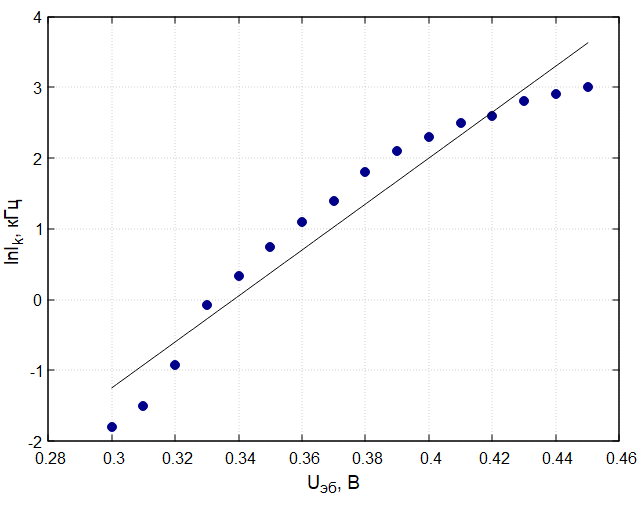
\includegraphics[width=0.8\textwidth]{Plot1.png}
\caption{График зависимости $\ln I_k = \ln I_0 + \frac{e}{kT}U_{\text{эб}}$ для таблицы \hyperref[tabl:1]{1}}
\label{fig:plot1}
\end{figure}

\begin{figure}
\centering
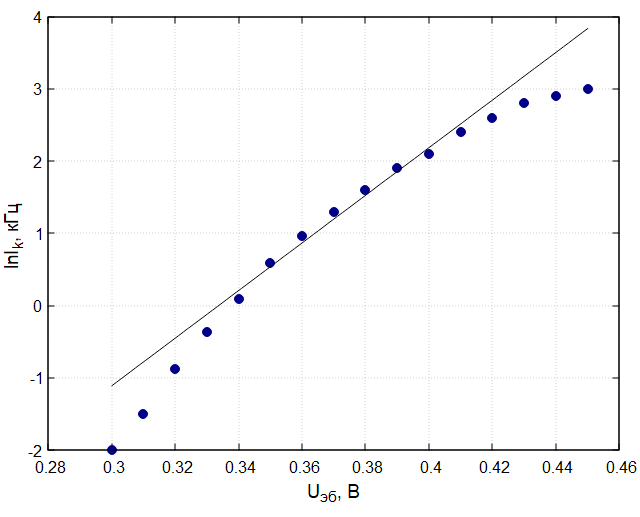
\includegraphics[width=0.8\textwidth]{Plot2.png}
\caption{График зависимости $\ln I_k = \ln I_0 + \frac{e}{kT}U_{\text{эб}}$ для таблицы \hyperref[tabl:2]{1'}}
\label{fig:plot2}
\end{figure}

\begin{figure}
\centering
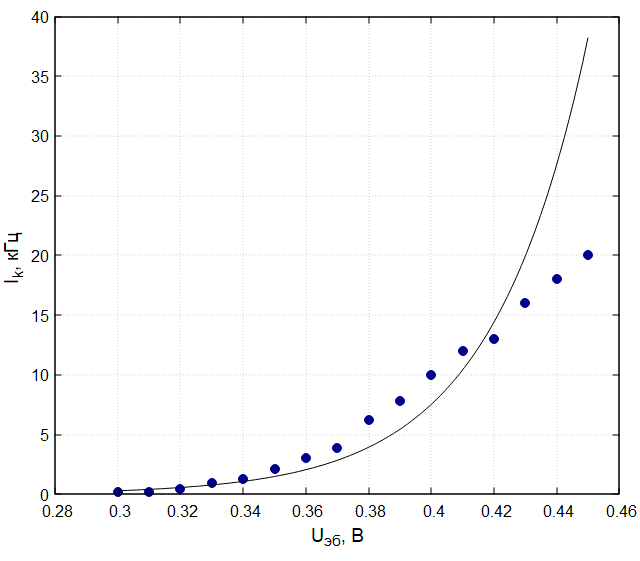
\includegraphics[width=0.8\textwidth]{Plot3.png}
\caption{График зависимости $I_k = I_0e^{\frac{eU_{\text{эб}}}{kT}}$ для таблицы \hyperref[tabl:2]{1}}
\label{fig:plot3}
\end{figure}

\begin{figure}
\centering
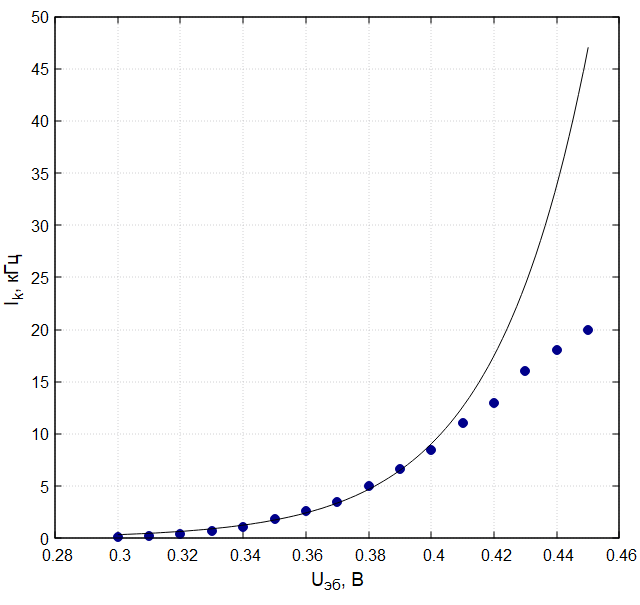
\includegraphics[width=0.8\textwidth]{Plot4.png}
\caption{График зависимости $I_k = I_0e^{\frac{eU_{\text{эб}}}{kT}}$ для таблицы \hyperref[tabl:2]{1'}}
\label{fig:plot4}
\end{figure}

\section{Вывод}
В ходе данной лабораторной работы были измерены напряжение между коллектором и базой биполярного транзистора с разной точностью и ток короткого замыкания коллектора, зависящие от напряжения между эмиттером и базой. Было определено отношение заряда электрона к постоянной Больцмана с погрешностью на основе полученных в ходе эксперимента, а также высчитанных далее значений. Построены графики зависимости $\ln I_k = \ln I_0 + \frac{e}{kT}U_{\text{эб}}$ и $I_k = I_0e^{\frac{eU_{\text{эб}}}{kT}}$ с нанесёнными на них точками полученных значений $\ln I_k$ от $U_{\text{эб}}$ и $I_k$ от $U_{\text{эб}}$ соответственно.

\begin{thebibliography}{9}
\bibitem{repo}
\url{https://github.com/st117208/Workshop1}  (дата обращения: 28.03.2025)
\end{thebibliography}